\begin{minipage}[t]{0.495\textwidth}
\centering
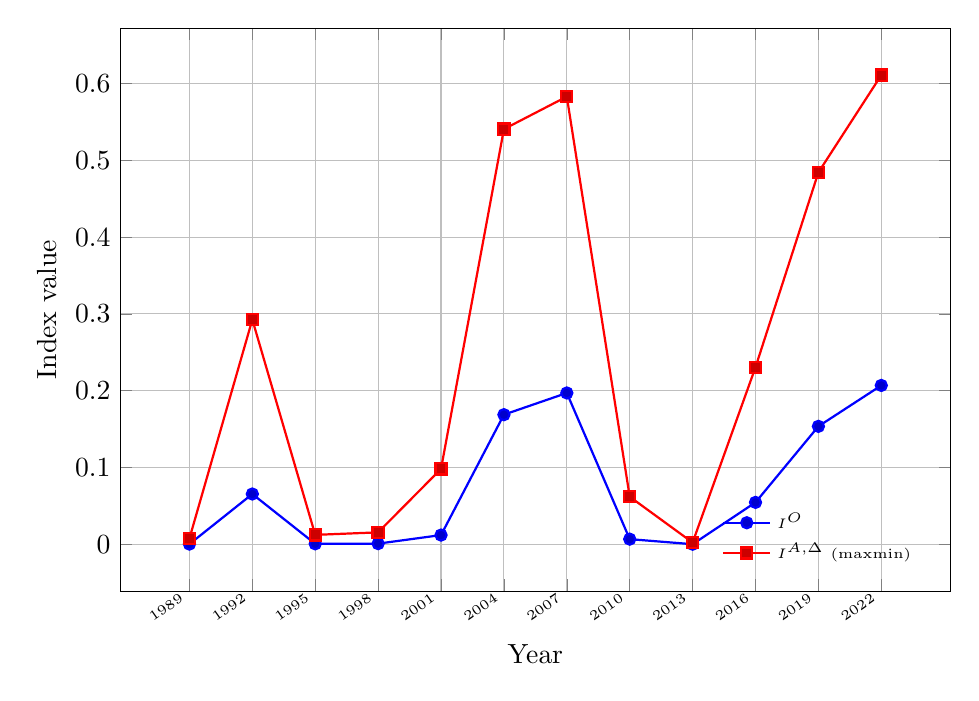
\begin{tikzpicture}
\begin{axis}[
width=\textwidth,
height=0.72\textwidth,
xlabel={Year},
ylabel={Index value},
legend pos=south east,
legend style={font=\tiny,draw=none,fill=none,cells={anchor=west}},
grid=major,
scaled x ticks=false,
xtick={1989,1992,1995,1998,2001,2004,2007,2010,2013,2016,2019,2022},
xticklabel style={/pgf/number format/fixed,/pgf/number format/precision=0,/pgf/number format/1000 sep={},rotate=35,anchor=east,font=\tiny},
]
\addplot+[thick, blue] coordinates {(1989, 0.00018965) (1992, 0.06541339) (1995, 0.00052918) (1998, 0.00079220) (2001, 0.01193740) (2004, 0.16874290) (2007, 0.19700426) (2010, 0.00664012) (2013, 0.00002643) (2016, 0.05450328) (2019, 0.15353819) (2022, 0.20682580)};
\addlegendentry{$I^{O}$}
\addplot+[thick, red] coordinates {(1989, 0.00756962) (1992, 0.29257416) (1995, 0.01221109) (1998, 0.01546825) (2001, 0.09813723) (2004, 0.54063652) (2007, 0.58300015) (2010, 0.06186573) (2013, 0.00219162) (2016, 0.23051601) (2019, 0.48425987) (2022, 0.61095209)};
\addlegendentry{$I^{A,\Delta}$ (maxmin)}
\end{axis}
\end{tikzpicture}
\end{minipage}
\hfill
\begin{minipage}[t]{0.495\textwidth}
\centering
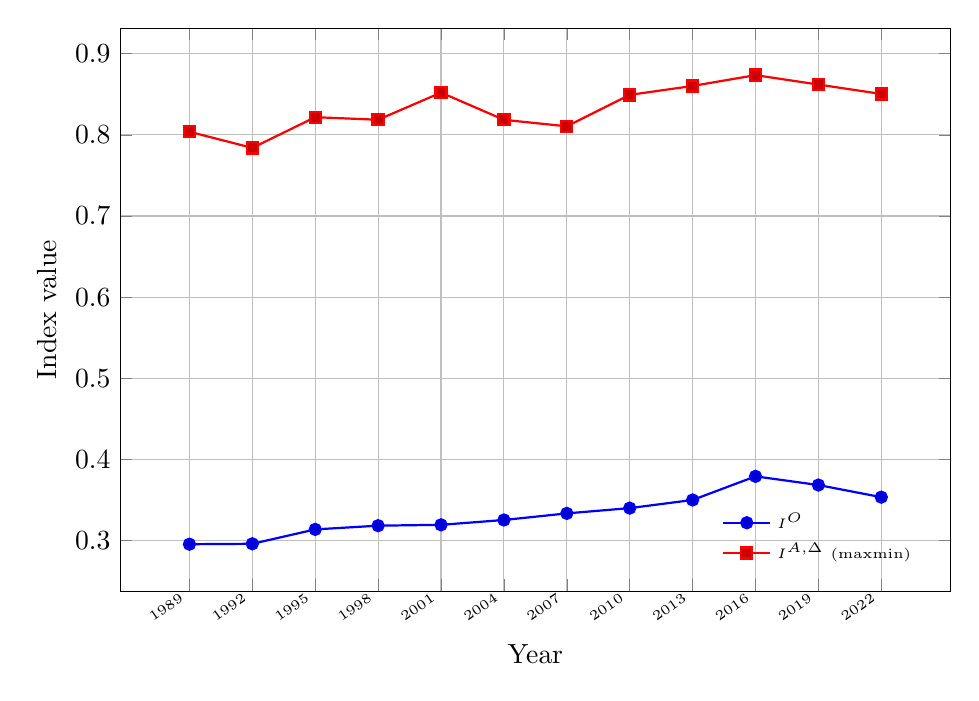
\begin{tikzpicture}
\begin{axis}[
width=\textwidth,
height=0.72\textwidth,
xlabel={Year},
ylabel={Index value},
legend pos=south east,
legend style={font=\tiny,draw=none,fill=none,cells={anchor=west}},
grid=major,
scaled x ticks=false,
xtick={1989,1992,1995,1998,2001,2004,2007,2010,2013,2016,2019,2022},
xticklabel style={/pgf/number format/fixed,/pgf/number format/precision=0,/pgf/number format/1000 sep={},rotate=35,anchor=east,font=\tiny},
]
\addplot+[thick, blue] coordinates {(1989, 0.29573316) (1992, 0.29625199) (1995, 0.31397152) (1998, 0.31857318) (2001, 0.31961987) (2004, 0.32556197) (2007, 0.33369668) (2010, 0.34020138) (2013, 0.35021353) (2016, 0.37932131) (2019, 0.36862002) (2022, 0.35366913)};
\addlegendentry{$I^{O}$}
\addplot+[thick, red] coordinates {(1989, 0.80375461) (1992, 0.78386219) (1995, 0.82171513) (1998, 0.81855865) (2001, 0.85200699) (2004, 0.81848044) (2007, 0.81044949) (2010, 0.84919180) (2013, 0.86018202) (2016, 0.87350944) (2019, 0.86188150) (2022, 0.85033816)};
\addlegendentry{$I^{A,\Delta}$ (maxmin)}
\end{axis}
\end{tikzpicture}
\end{minipage}

{\footnotesize $I^{A,\pi}$ with singleton $C=\{\pi_t\}$ equals $I^{O}$ (audit CSV: columns I\_O and I\_A\_singleton).}

% Net Wealth inequality measures
